\documentclass{article}
\usepackage[T1]{fontenc}
\usepackage[utf8]{inputenc}
\usepackage{lmodern}
\usepackage{cancel}
\usepackage{graphicx,pict2e}
\usepackage{fancybox,multido}
\usepackage{amsmath}
\usepackage{pgfplots}
\usepackage{mathtools}

\title{Obliczenia Naukowe\\Ćwiczenia}
\author{Jakub Kowal}
\date{}

\begin{document}
\maketitle
\renewcommand{\thesubsubsection}{\thesubsection.\alph{subsubsection})}

    \section{Lista 1}
    \subsection{}
    $a_{1}=0,25$    $\tilde{a_{1}} = 0,25 * 10^{0}$\\
    $a_{2}=0,0046$    $\tilde{a_{2}} = 0,46 * 10^{-2}$\\
    $a_{3}=0,00079$    $\tilde{a_{3}} = 0,79 * 10^{-3}$\\
    $a_{4}=0,061$    $\tilde{a_{4}} = 0,61 * 10^{-1}$\\
    $((\tilde{a_{1}}\oplus \tilde{a_{2}})\oplus \tilde{a_{3}})\oplus \tilde{a_{4}}$\\
    $\tilde{a_{1}}\oplus \tilde{a_{2}} = 0,25 * 10^{0}\oplus 0,46 * 10^{-2}=0,25 * 10^{0} \oplus 0,0046 * 10^{0} = rd(0,2546*10^{0})= 0,25 * 10^{0}=\tilde{a_{12}}$\\
    $\tilde{a_{12}}\oplus \tilde{a_{3}} = 0,25 * 10^{0} \oplus 0,79*10^{-3} = rd(0,25079*10^{0}) = 0,25 * 10^{0}= \tilde{a_{123}}$\\
    $\tilde{a_{123}} \oplus \tilde{a_{4}} = 0,25 * 10^{0} \oplus 0,61*10^{-1}=rd(0,311*10^{0})=0,31*10^{0}$\\
    $((\tilde{a_{3}}\oplus \tilde{a_{2}})\oplus \tilde{a_{4}})\oplus \tilde{a_{1}}$\\
    $\tilde{a_{3}}\oplus \tilde{a_{2}} = 0,54*10^{-2}$\\
    $\tilde{a_{32}}\oplus \tilde{a_{4}} = 0,66*10^{-1}$\\
    $\tilde{a_{432}} \oplus \tilde{a_{1}} = 0,32 * 10^{0}$\\
    Wynik rzeczywisty = 0,31639\\
    $\delta = \frac{|0,31639 - 0,31|}{|0,31369|}=0,0201966$\\
    $\delta = \frac{|0,31639 - 0,32|}{|0,31369|}=0,01141$

    \subsection{}
    \subsubsection{}
    $x=0,54617$ $\tilde{x}=0,5462$\\
    $y=0,54601$ $\tilde{y}=0,5460$\\
    $r=x-y=0,00016$ $\tilde{r}=\tilde{x} \ominus \tilde{y}=rd(0,00016)=0,2*20^{-3}$\\
    $\epsilon = 0,5 \beta^{1-t}=0,5 * 10^{-3}$\\

    \subsubsection{}
    $\beta = 10$ $t = 3$\\
    $a=1,22$\\
    $b=3,34$\\
    $c=2,28$\\
    \begin{math}
        \tilde{\Delta}=\tilde{b} \odot \tilde{b}\ominus 4\odot \tilde{a}\odot \tilde{c}=rd(3,34*3,34)\ominus \dots =11,16\ominus4\odot \tilde{a}\odot \tilde{c}= 0,4 * 10^{1}\odot 0,122*10^{1}=(0,488*10^{-1})\\
        (0,488*10^{1})\odot (0,228 * 10^{1})=(0,111*10^{2})\\
        \tilde{\Delta}=(0,112*10^[2])\ominus (0,111*10^{2})=(0,001*10^{2})=0,1\\
        \Delta = 0,0292\\
        \frac{|\Delta - \tilde{\Delta}|}{|\Delta|}=\frac{|0,0292-0,1|}{|\Delta|}=2,42\\
        \epsilon = \frac{1}{2}\beta^{1-t}=\frac{1}{2}*10^{-2}=0,005
    \end{math}

    \subsection{}
    \begin{math}
        (0,78125)_{10}=(0,11001)_{2}\\
        z=\pm m_{z} 2^{c} m_{z}\in [\frac{1}{2},1)\\
        0,11001*2^{0}\\
        0,101111001*2^{10}\\
        (754)_{10} = (1011110010)_{2}
    \end{math}
    
    \subsection{}
    \subsubsection{}
    \begin{math}
        t=23\\
        n\in [1,2)\\
        x=2^{-1}+2^{-26}\\
        2^{-1}=(\frac{1}{2})_{10}=(0,1)_{2}\\
        2^{-26}=(\frac{1}{2^{26}})_{10}=(0,\underbrace{0\dots0}_{\text{25}}1)_{2}\\
        x=0,1\underbrace{0\dots0}_{\text{24}}1\\
        \tilde{x}=1,\underbrace{0\dots0}_{\text{24}}1*2^{-1}
    \end{math}
    Odp. Nie

    \subsubsection{}
    \begin{math}
        y=\frac{1}{3}=0,(3)\\
        \tilde{y}=1,(01)_{2}*2^{-2}\\
        0,(3)=0,(01)_{2}\\
        0,(3)*2\\
        0,(6)*2\\
        1,3*1
    \end{math}
    Odp. Nie

    \subsubsection{}
    \begin{math}
        z=\frac{1}{5}=0,2\\
        \tilde{z}=1,(0011)*2^{-3}
    \end{math}
    Odp. Nie

    \subsubsection{}
    \begin{math}
        j=\frac{1}{10}=(0,1)_{10}\\
        0,1*2\\
        \tilde{j}=1,(00011)_{2}*2^{-4}
    \end{math}
    
    \subsection{}
    33-bitowe słowo $x=sm2^{c}$\newline
    cecha 8 bitów ze znakiem\newline
    mantysa 24 bity $\in [\frac{1}{2},1)$\newline
    
    \subsubsection{}
    $x_{max}=(0.11...1)_{2}*2^{127}=(1-2^{-24})*2^{127}=1,7*10^{38}$\newline
    $x_{min}=(0.10...0)_{2}*2^{-127}=2^{-1}*2^{-127}=2^{-128}$\newline
    $[-x_{max},-x_{min}]\cup[x_{min},x_{max}]$\newline
    
    \subsubsection{}
    $(-x_{min},x_{min})$\newline
    
    \subsubsection{}
    $\epsilon=\frac{1}{2}*\beta^{1-t}=2^{-1}*2^{-23}=2^{-24}$
    
    \subsection*{Single}
    \setcounter{subsubsection}{0}
    \subsubsection{}
    $x_{max}=(2*2^{-23})*2^{127}\approx3,4*10^{38}$\newline
    $x_{min}=1*2{-126}=2^{-126}$\newline
    $x_{minsub}=(0.00.....01)_{2}*2^{-126}=2^{-23}*2^{-126}=2^{-149}$\newline
    $[-x_{max},-x_{min}]\cup\{0\}\cup[x_{min},x_{max}]$\newline
    
    \subsubsection{}
    $(-x_{minsub},x_{minsub})$\newline

    \subsubsection{}
    $\epsilon=\frac{1}{2}\beta^{1-t}=2^{-1}*2^{-23}=2^{-24}$\newline

    \subsection{}
    \subsubsection{}
    x = $1+2^{-24}$\newline
    $\epsilon = 2^{-23}$\newline
    $x^{-} = 1$\newline
    $x^{+} = 1 + 2^{-23}$\newline
    
    \subsubsection{}
    $x \bigoplus 1 = 1$\newline
    $x \in (0,2^{-24}+2^{-25}]$\newline
    
    \subsubsection{}
    $x \bigoplus =x$\newline
    $x<\frac{x}{2^{23}}$

    \subsection{}

    % \fancyput(3.25in,-4.5in){%
    % \setlength{\unitlength}{1in}\fancyoval(7,10)}
    % \multido{\iA=1+1}{20}{\fbox{\includegraphics[page=\iA,scale=0.75]{/home/kuba/Projects/Sem-5/Obliczenia Naukowe/listy/scnal1cw.pdf}}\par}

    $A(a_{1},...,a_{n})=(...(a_{1}\oplus a_{2})\oplus a_{3})\oplus ...)\oplus a_{n} = (...(a_{1}+a_{2})(1+\delta_{1})+a_{3})(1+\delta_{2})+...)+a_{n})(1+\delta_{n-1})=a_{1}+a_{1}*E_{1}+a_{2}+a_{2}*E_{1}+a_{3}+a_{3}*E_{2}...+a_{n}+a_{n}*E_{n-1}=(a_{1}+a_{2}+...+a_{n})+(a_{1}*E_{1}+a_{2}*E_{1}+...+a_{n}*E_{n-1})=S+(a_{1}*E_{1}+a_{2}*E_{1}+...+a_{n}*E_{n-1})$\newline
    $|\delta|\le\epsilon$\newline 
    $1+E_{k}=\prod_{i=1}^{k}(1+\delta_{k})\leftarrow wprowadzamy$\newline
    $(a_{1}*E_{1}+a_{2}*E_{1}+...+a_{n}*E_{n-1})=E_{max}=\prod_{i=1}^{n-1}(1+|\delta_{i}|)-1\le \prod_{i=1}^{n-1}(1+\epsilon)-1$\newline
    $a_{1}*E_{1}+a_{2}*E_{1}+...+a_{n}*E_{n-1}\le (a_{1}+a_{2}+...+a_{n})*E_{max}\le ((a_{1}+a_{2}+...+a_{n})*\prod_{i=1}^{n-1}(1+\epsilon))-1 = S(1+\epsilon)^{n-1}-1$\newline
    $\frac{|\tilde{S}-S|}{|S|}\le \frac{\cancel{S}+S*(1+s)}{|S|} \leftarrow$ Zmazał za szybko\newline
    $\tilde{S}\le S+S*(1+\epsilon)^{n-1}-1$
    
    \subsection{}
    P(n-1)=$\prod_{i=0}^{n-1}q_{i}$ --- dokładny wynik\\
    Q(n-1)=fl(P(n-1)) ---wynik w fl\\
    Q(n-1)=$P(n-1)(1+\sum_{i=1}^{n-1}q_{i}), \forall i |\delta_{i}|\le \epsilon$  
    n=1 Q(1)=$a_{0}\odot a_{1}=a_{0}a_{1}(1+\delta_{1})=P(1)(1+\sum_{i=1}^{1}q_{i})$\\
    Zachodzi dla 1\\
    Q(n+1)=$a_{0}\odot a_{1}\odot \cdots \odot a_{n+1}$=Q(n)$\odot a_{n+1}=(Q(n)a_{n+1})(1+\delta_n+1)=P(n)(1+\sum_{i=1}^{n})a_{n+1}(1+\delta_{n+1})=P(n+1)(1+\sum_{i=1}^{n}\delta_{1})(1+\delta_{n+1})\approx P(n+1)(1+\delta_{n+1}+\sum_{i=1}^{n}\delta_{i})=P(n+1)(1+\sum_{i=1}^{n+1}\delta_{i})$\\
    \begin{flushright}
        % $\Box$ 
    \end{flushright}
    |P(n)-Q(n)|=$|P(n)\sum_{i=1}^{n}\delta_{i}|$


    \subsection{}
    $A1(a,b) = a^{2}-b^{2}$\\
    $fl(a^{2}-b^{2})=fl(fl(a^{2})-fl(b^{2}))=(a^{2}(1+\delta_{1})-b^{2}(1+\delta_{2}))(1+\delta_{3})\approx a^{2}-b^{2}+(a^{2}-b^{2})\delta_{3}+a^{2}\delta_{1}-b^{2}\delta_{2}$\\
    Błąd względny:\\
    $\frac{|a^{2}-b^{2}+(a^{2}-b^{2})\delta_{3}+a^{2}\delta_{1}-b^{2}\delta_{2}-(a^{2}-b^{2})|}{|a^{2}-b^{2}|}= \frac{|(a^{2}-b^{2})\delta_{3}+a^{2}\delta_{1}-b^{2}\delta_{2}|}{|a^{2}-b^{2}|}\le |\delta_{3}|+ \frac{|a^{2}\delta_{1}-b^{2}\delta_{2}|}{|a^{2}-b^{2}|}\le |\delta_{3}|+ \frac{a^{2}|\delta_{1}|-b^{2}|\delta_{2}|}{|a^{2}-b^{2}|} \le \epsilon + \frac{a^{2}\epsilon + b^{2}\epsilon}{|a^{2}-b^{2}|}=\epsilon(1+\frac{a^{2}+b^{2}}{|a^{2}-b^{2}|})$\\
    $A2(a,b)=(a-b)(a+b)$\\
    $((a-b)(1+\delta_{1})(a+b)(1+\delta_{2}))(1+\delta_{3})= (a^{2}-b^{2})(1+\delta_{1})(1+\delta_{2})(1+\delta_{3})\approx (a^{2}-b^{2})(1+\delta_{1}+\delta_{2}+\delta_{3})$\\
    Błąd względny:\\
    $\frac{|(a^{2}-b^{2})(1+\delta_{1}+\delta_{2}+\delta_{3})-(a^{2}-b^{2})|}{|a^{2}-b^{2}|}=|\delta_{1}+\delta_{2}+\delta_{3}|\le |\delta_{1}|+|\delta_{2}|+|\delta_{3}|\le 3\epsilon$

    \section{Lista 2}
    
    \subsection{}
    $y=\sqrt{x^{2}+1}-1$\newline
    TW z wykładu:\newline
    Jeśli x,y - dodatnie liczby w dwójkowej arytmetyce float, takie że:\newline
    $x>y, 2^{-q}\le 1-\frac{y}{x}$\newline
    to przy odejmowaniu tracimy najwyżej q bitów q = 2\newline
    $2^{-2}\le 1-\frac{1}{\sqrt{x^{2}+1}}$\newline
    $\frac{1}{4}=1-\frac{1}{\sqrt{x^{2}+1}}$\newline
    $\frac{1}{\sqrt{x^{2}+1}}\le \frac{3}{4}$\newline
    $\sqrt{x^{2}+1}>=\frac{3}{4}$\newline

    \subsection{}
    Wskazówka:\\
    Twierdzenie z 1 zadania:
    $2^{-q}<=1-\frac{a}{b}<=2^{-P}$ $\land$ $b-a, b>a$\\
    $x=\frac{1}{2}$\\
    $\cos \frac{1}{2}=0,8775825$\\
    $2^{-q}<=1-\frac{0,8775825}{1}<=2^{-P}$\\
    $2^{-q}<=0,1224175<=2^{-P}$\\
    $q=4 \land P=3$


    \subsection{}
    f(x)=$x^{-1}(1-\cos x)$\\
    a) $\lim_{x \rightarrow 0}\frac{1-\cos x}{x}(De'Hospital)=\lim_{x\rightarrow 0}\frac{\sin x}{1}=0$\\
    b) $\cos x\approx 1$\\
    $x\approx 2\pi k, k \in Z$\\
    $1-\cos x = 2\sin^{2}\frac{x}{2}$\\
    f(x)=$\frac{2\sin^{2}\frac{x}{2}}{x}=(t=\frac{x}{2})=\frac{\cancel{2}\sin^{2}t}{\cancel{2}t}=t(\frac{\sin t}{t})^{2}=\frac{x}{2}(\frac{\sin\frac{x}{2}}{\frac{x}{2}})^{2}$\\
    $\lim_{x\rightarrow0}\frac{\sin t}{t}=1$ dla $x\rightarrow 0(t\rightarrow 0)$ mamy $f(t)=t1^{2}=t=\frac{x}{2}$\\
    
    \subsection{}
    $f(x)=\sqrt{x+2}-\sqrt{x}$\newline
    Problem dla dużych x : $\sqrt{x}\approx\sqrt{x+2}$\newline
    $\sqrt{x+2}-\sqrt{x} /*\frac{\sqrt{x+2}+\sqrt{x}}{\sqrt{x+2}+\sqrt{x}}$\newline
    $\frac{x+2-x}{\sqrt{x+2}+\sqrt{x}}=\frac{2}{\sqrt{x+2}+\sqrt{x}}$\newline
    $a^{2}-b^{2}=(a-b)(a+b)$\newline

    \subsection{}
    \begin{math}
        u=\pm \sqrt{\frac{x+\sqrt{x^{2}+y^{2}}}{2}}\\
        v=\frac{y}{2u}\\
        liczba zespolona= x + iy\\
        x\ne 0\\
        pierwiastek to u+iv\\
        x\ge 0 : \text{jeśli y<<x, to może dojść do ''pochłonięcia'' y}\\
        \text{poza tym dokładność generalnie dobra}\\
        x<0 : \text{może się zdarzyć, że } |x|\approx \sqrt{x^{2}+y^{2}}\\
        \text{i nastąpi utrata cyfr znaczących w liczniku, więc dokładność wzoru jest słaba}\\
        \text{alternatywny wzór na } k<0:\\
        x+\sqrt{x^{2}+y^{2}}=\frac{(x+\sqrt{x^{2}+y^{2}})(x-\sqrt{x^{2}+y^{2}})}{(x-\sqrt{x^{2}+y^{2}})}=\frac{x^{2}-x^{2}-y^{2}}{x-\sqrt{x^{2}+y^{2}}}=\frac{-y^{2}}{x-\sqrt{x^{2}+y^{2}}}=\frac{-y^{2}}{-(|x|+\sqrt{x^{2}+y^{2}})}\\
        \text{Wtedy }u=\sqrt{\frac{-y^{2}}{2(x-\sqrt{x^{2}+y^{2}})}}=\sqrt{\frac{y^{2}}{2(|x|+\sqrt{x^{2}+y^{2}})}}
    \end{math}

    \subsection{}
    $4ac\rightarrow0$\\
    x=$\frac{-b\mp \sqrt{b^{2}-4ac}}{2a}$\\
    $x_{1}x_{2}=\frac{c}{a}$
    $q=\frac{1}{2a}(-b-sqm?(b)\sqrt{b^{2}-4ac})$\\
    $x_{1}=\frac{-b+\sqrt{b^{2}-4ac}}{2a}$\\
    $x_{2}=\frac{-b-\sqrt{b^{2}-4ac}}{2a}=\frac{-(b+\sqrt{b^{2}-4ac})}{2a}$\\
    $x_{1}=\frac{c}{ax_{2}}$\\
    \begin{flushright}
        \parbox{100mm}{
            $b=0    ax^{2}+c=0\\\Delta=-4ac$
        }
    \end{flushright}
    $b< 0 $\\
    $x_{1}=\frac{|b|+\sqrt{b^{2}-4ac}}{2a}$\\
    $x_{2}=\frac{c}{2a}$

    \setcounter{subsection}{7}

    \subsection{}
    $\frac{|f(\hat{x})-f(x)|}{|f(x)|}=\frac{|f(x+x\delta)-f(x)|}{|f(x)|}\approx \frac{|f`(x)x\delta|}{|f(x)|}=cond(x)|\delta|$\\
    $x^{\alpha}   (x^{\alpha})`=\alpha x^{\alpha-1}       \frac{|(\alpha x^{alpha-1})x\delta|}{|x^{\alpha}|}=\frac{|\alpha x^{\alpha}\delta|}{|x^{\alpha}|}=\alpha \delta$\\
    $\sin x (\sin x)`=\cos x      \frac{|(\cos x)x\delta|}{|\sin x|}=\frac{x\delta}{\tan x}$\\
    $e^{x} (e^{x})`=e^{x}$\\
    $x^{-1}e^{x} (x^{-1}e^{x})`=x^{-1}e^{x}+(-1)x^{-2}e^{x}=\frac{e^{x}}{x}-\frac{e^{x}}{x^{2}}$\\
    $\arcsin x$

    \section{Lista 3}

    \subsection{}
    Bisekcji [$a_{0},b_{0}$] $c_{n}=\frac{a_{n}+b_{n}}{2}$\\
    \begin{math}
        \lim_{n \rightarrow \infty} c_{n}=r\\
        e_{n}=r-c_{n}\\
    \end{math}
    \subsubsection{}
    \begin{math}
        f(x)=x-10\\
        \text{Czy relacja } |e_{0}|\ge |e_{1}| \ge \dots\\
        r=10\\
        f(10)=0\\
        a_{0}=0\\
        b_{0}=22\\
        c_{0}=11\\
        e_{0}=-1\\
        |e_{0}|=1\\
        a_{1}=0\\
        b_{1}=11\\
        c_{1}=5.5\\
        e_{1}=4.5\\
        |e_{0}|<|e_{1}|\\
    \end{math}
    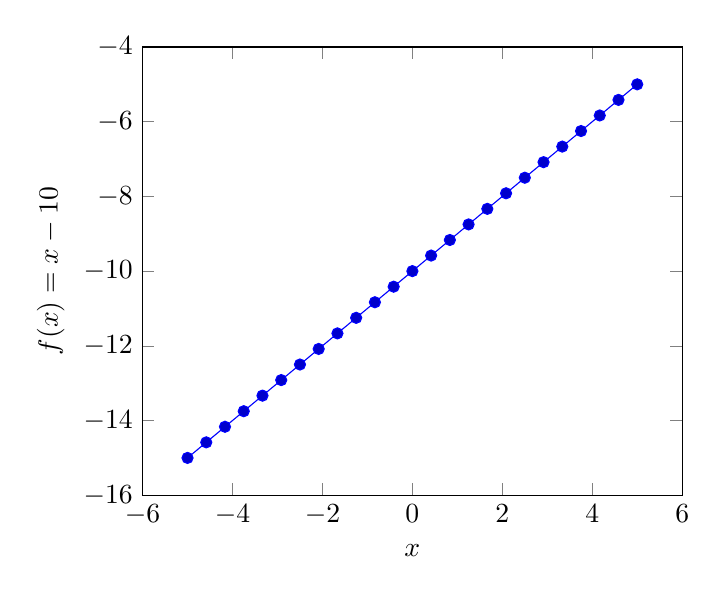
\begin{tikzpicture}
    \begin{axis}[ 
        xlabel=$x$,
        ylabel={$f(x) = x-10$}
    ] 
        \addplot {x-10}; 
    \end{axis}
    \end{tikzpicture}
    \subsubsection{}
    % \begin{math}
    %     \text{Pokaż, że }[a_{n},b_{n}]\supseteq[a_{n+1},b_{n+1}]\forall n\ge 0\\
    %     |e_{0}|<|e_{1}|\\
    %     n=0 \\
    %     a_{0}\le b_{0}\\
    %     c_{0}=\frac{a_{0}+b_{0}}{2}\\
    %     n=1\\
    %     [a_{1},b_{1}]=\begin{cases*}
    %             [a_{0},\frac{a_{0}+b_{0}}{2}]& f(a_{0})f(a_{0}+b_{0})\le 0\\
    %             [a_{0},\frac{a_{0}+b_{0}}{2}]& f(a_{0})f(a_{0}+b_{0})\le 0
    %         \end{cases*}
    % \end{math}

\end{document}